%%%%%%%% ICML 2025 EXAMPLE LATEX SUBMISSION FILE %%%%%%%%%%%%%%%%%

\documentclass{article}

% Recommended, but optional, packages for figures and better typesetting:
\usepackage{microtype}
\usepackage{graphicx}
\usepackage{subfigure}
\usepackage{booktabs} % for professional tables

% hyperref makes hyperlinks in the resulting PDF.
% If your build breaks (sometimes temporarily if a hyperlink spans a page)
% please comment out the following usepackage line and replace
% \usepackage{icml2025} with \usepackage[nohyperref]{icml2025} above.
\usepackage{hyperref}

% Attempt to make hyperref and algorithmic work together better:
\newcommand{\theHalgorithm}{\arabic{algorithm}}

% Use the following line for the initial blind version submitted for review:
% \usepackage{icml2025}

% If accepted, instead use the following line for the camera-ready submission:
\usepackage[accepted]{icml2025}

% For theorems and such
\usepackage{amsmath}
\usepackage{amssymb}
\usepackage{mathtools}
\usepackage{amsthm}

% % For code
% \usepackage{listings}
% \usepackage[frozencache,cachedir=.]{minted}

% if you use cleveref..
\usepackage[capitalize,noabbrev]{cleveref}

%%%%%%%%%%%%%%%%%%%%%%%%%%%%%%%%
% THEOREMS
%%%%%%%%%%%%%%%%%%%%%%%%%%%%%%%%
\theoremstyle{plain}
\newtheorem{theorem}{Theorem}[section]
\newtheorem{proposition}[theorem]{Proposition}
\newtheorem{lemma}[theorem]{Lemma}
\newtheorem{corollary}[theorem]{Corollary}
\theoremstyle{definition}
\newtheorem{definition}[theorem]{Definition}
\newtheorem{assumption}[theorem]{Assumption}
\theoremstyle{remark}
\newtheorem{remark}[theorem]{Remark}

% Todonotes is useful during development; simply uncomment the next line
%    and comment out the line below the next line to turn off comments
%\usepackage[disable,textsize=tiny]{todonotes}
% \usepackage[textsize=tiny]{todonotes}


% The \icmltitle you define below is probably too long as a header.
% Therefore, a short form for the running title is supplied here:
\icmltitlerunning{Re-Examine Hybrid State-Space and Self-Attention for In-Context Learning}

\begin{document}

\twocolumn[
\icmltitle{Re-Examine Hybrid State-Space and Self-Attention for In-Context Learning}

% It is OKAY to include author information, even for blind
% submissions: the style file will automatically remove it for you
% unless you've provided the [accepted] option to the icml2025
% package.

% List of affiliations: The first argument should be a (short)
% identifier you will use later to specify author affiliations
% Academic affiliations should list Department, University, City, Region, Country
% Industry affiliations should list Company, City, Region, Country

% You can specify symbols, otherwise they are numbered in order.
% Ideally, you should not use this facility. Affiliations will be numbered
% in order of appearance and this is the preferred way.
\icmlsetsymbol{equal}{*}

\begin{icmlauthorlist}
\icmlauthor{Jingze Shi}{equal,IR}
\icmlauthor{Bingheng Wu}{equal,IR}
\end{icmlauthorlist}

\icmlaffiliation{IR}{Independent Researcher}


\icmlcorrespondingauthor{Jingze Shi}{losercheems@gmail.com}
\icmlcorrespondingauthor{Bingheng Wu}{wubingheng52136@gmail.com}

% You may provide any keywords that you
% find helpful for describing your paper; these are used to populate
% the "keywords" metadata in the PDF but will not be shown in the document
\icmlkeywords{Machine Learning, ICML}

\vskip 0.3in
]



\begin{abstract}
% 最近的研究表明, 将状态空间算法驱动的 Mamba 与自注意力算法驱动的 Transformer 相结合, 在大多数语言建模任务上的表现超越了单独使用 Mamba 或 Transformer. 
% 但是, 目前主流的混合建模架构模型在情景学习任务上的表现并不理想, 我们重新审视了这两种算法的优势和劣势, 从原理出发对这种混合建模的结构重新设计. 
% 最终, 重新设计的架构, 在标准短文本任务中提升了 1.3 \% 效果, 在自然长文本任务中提升了 20.86 \% 效果, 在合成长文本任务中提升了 27.06 \% 效果.
Recent research has shown that combining the state-space algorithm-driven Mamba with the self-attention algorithm-driven Transformer outperforms using Mamba or Transformer alone in most language modeling tasks. However, the performance of the mainstream hybrid modeling architecture models in in-context learning tasks is not ideal. We re-examine the advantages and disadvantages of these two algorithms and redesign the structure of this hybrid modeling from the principle. The finally redesigned architecture improves the performance by 1.3\% in standard short text tasks, 20.86\% in natural long text tasks, and 27.06\% in synthetic long text tasks.
\end{abstract}

\section{Introduction}
\label{submission}
% Transformers~\cite{transformer2017} 架构的自注意力算法能够直接捕捉序列中任意两个元素间的关系, 有效处理长距离依赖问题. 但是却受到二次复杂度的限制.
% Mamba~\cite{gu2023mamba} 架构的状态空间算法能够在训练期间实现序列长度的线性缩放, 并在生成期间保持恒定的状态大小, 但是却在捕捉长距离依赖问题上导致偏差.
% 混合建模架构模型, 例如 Wonderful Matrices~\cite{shi2024wonderfulmatrices}, Jamba~\cite{lieber2024jamba}, 等等, 使用状态空间和自注意力进行混合建模, 使模型具备与 Mamba 类似的效率和与 Transformer 类似的效果. 然而, 这些模型在情景学习任务上的表现却与原始的 Transformer 相比, 仍然有不小的差距.
The self-attention algorithm of the Transformers~\cite{wolf-etal-2020-transformers} architecture can directly capture the relationship between any two elements in a sequence, effectively handle long-distance dependencies. However, it is limited by quadratic complexity. The state-space algorithm of the Mamba~\cite{gu2023mamba} architecture can achieve linear scaling of sequence length during training and maintain a constant state size during generation, but it leads to bias in capturing long-distance dependencies. Hybrid modeling architecture models, such as Wonderful Matrices~\cite{shi2024wonderfulmatrices}, Jamba~\cite{lieber2024jamba}, etc., use state-space and self-attention for hybrid modeling, making the model have efficiency similar to The Mamba and effect similar to The Transformer. However, these models still have a significant gap in performance in in-context learning tasks compared to the original Transformer.

% 我们提出了 Self-Attention before LM-Head~\ref{fig:architecture}, 这是对现有的混合堆叠架构模型的一种简单改变, 将状态空间和自注意力修改为使用相同的位置编码, 并在 LM-Head 预测概率分布之前使用自注意力和前馈网络构成的 Transformer 块. 这种方法使得模型能够继续利用状态空间的高效上下文摘要和自注意力有效联想召回的优势, 而不会在最终的token预测上产生偏差.
We propose Self-Attention before LM-Head~\ref{fig:architecture}, which is a simple change to the existing hybrid stacked architecture models, modifying the state-space and self-attention to use the same positional encoding, and using a Transformer block composed of self-attention and feed-forward networks before the LM-Head predicts the probability distribution. This method allows the model to continue to leverage the advantages of the efficient context summary of the state-space and the effective associative recall of self-attention without bias in the final token prediction.

% 我们的研究与评估表明, Self-Attention before LM-Head 只需要很少的结构与参数调整, 就能够与基线混合模型相比, 在上下文学习任务基准上取得更好的性能. 例如, 在标准短文本任务中, 我们的模型提升了 1.3 \% 的效果, 在自然长文本任务中提升了 20.86 \% 的效果, 在合成长文本任务中提升了 27.06 \% 的效果, 并且在大海捞针任务上取得了最先进的效果.
Our research and evaluation show that Self-Attention before LM-Head can achieve better performance on the in-context learning task benchmark compared to the baseline hybrid model with only a few structural and parameter adjustments. For example, in standard short text tasks, our model improves performance by 1.3\%, in natural long text tasks by 20.86\%, in synthetic long text tasks by 27.06\%, and achieves state-of-the-art performance on the needle in a haystack task.

\begin{figure*}[ht]
   \centering
   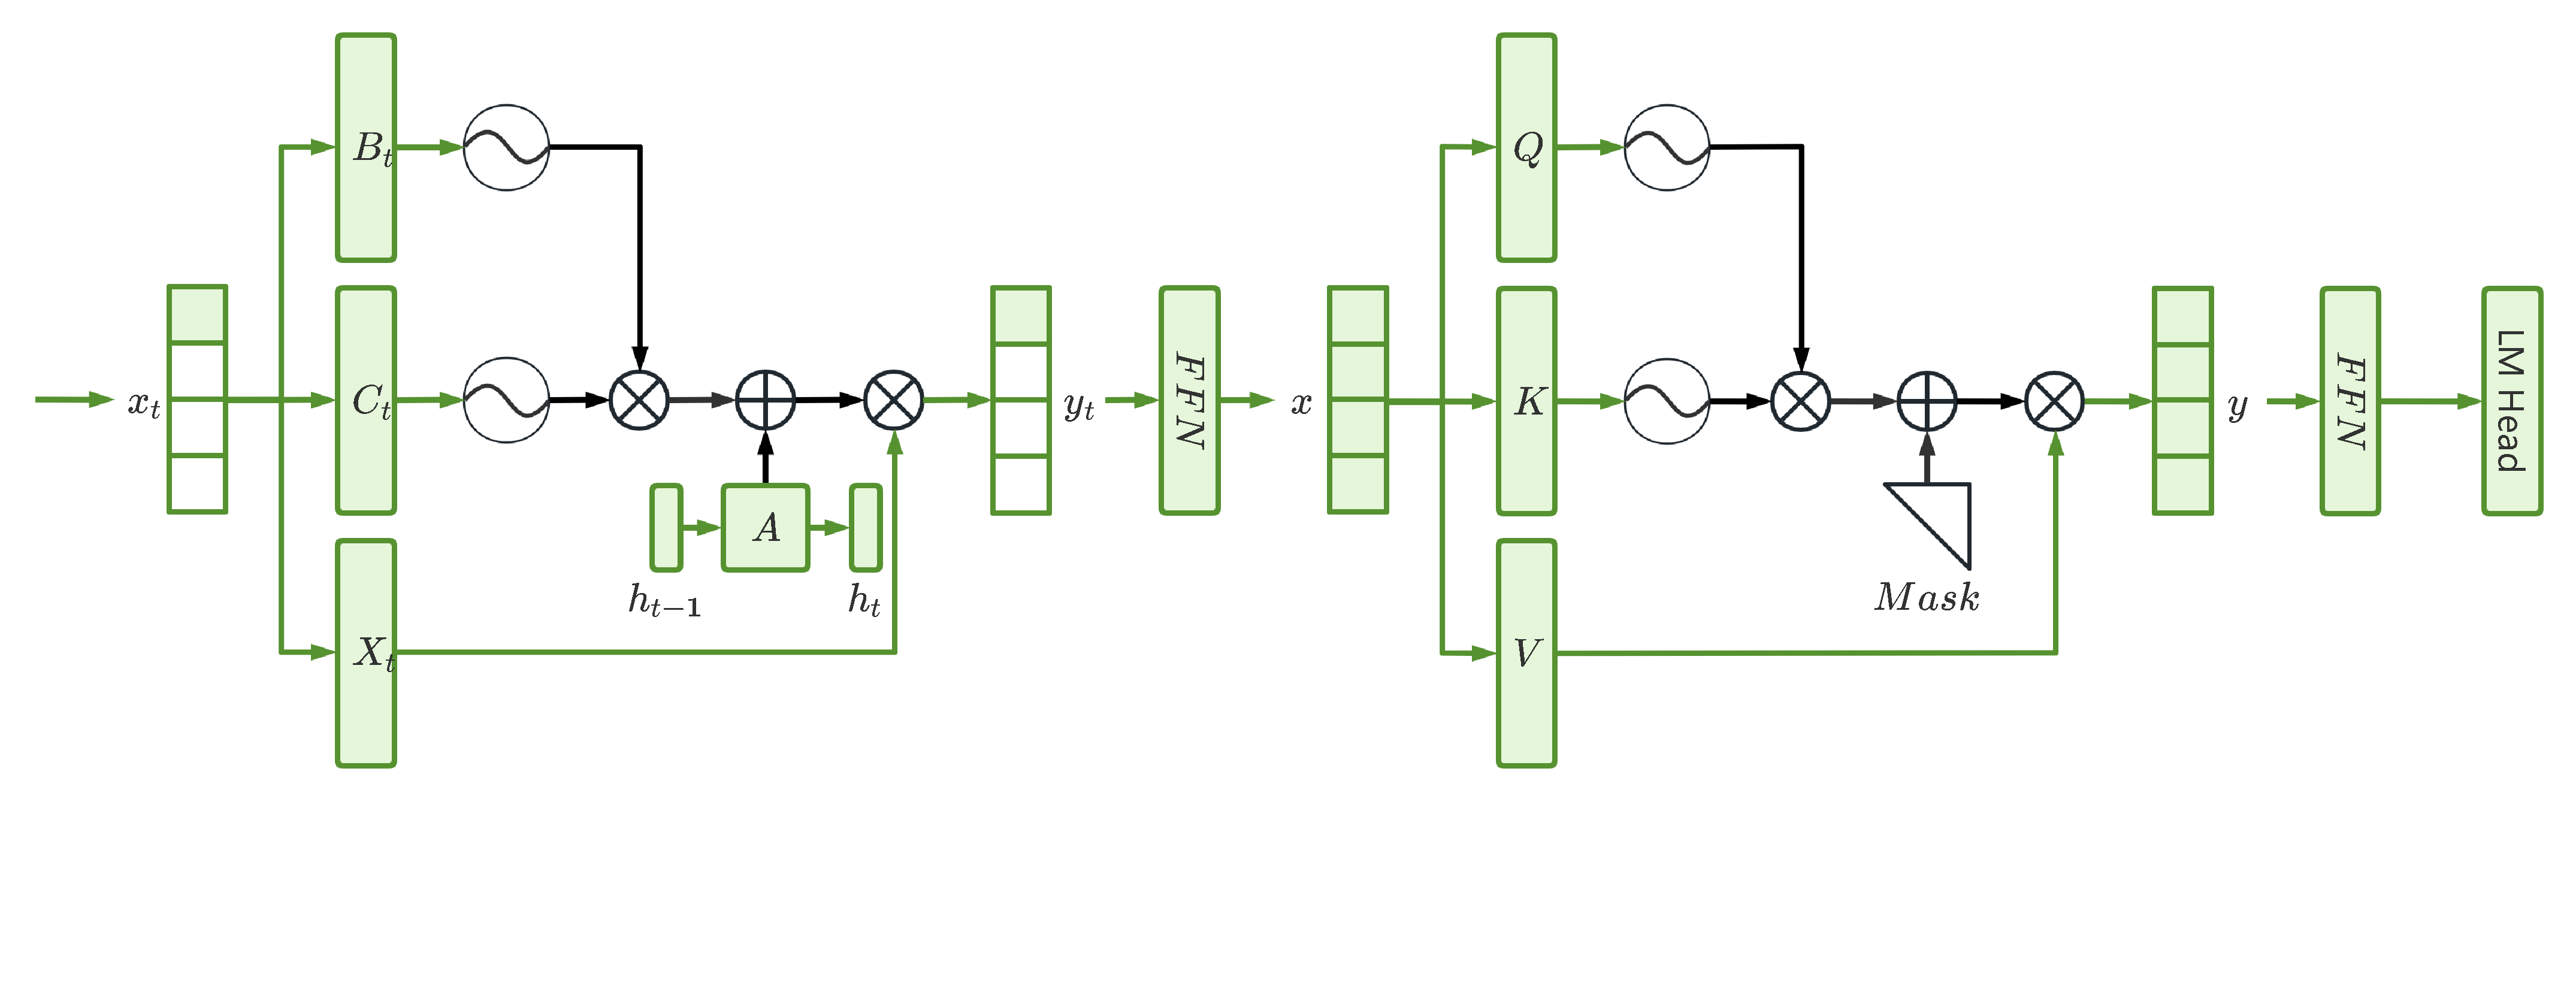
\includegraphics[width=\linewidth]{fig/architecture.pdf}
   \caption{
      % 状态空间和自注意力都使用相同的位置编码, 并且在 LM-Head 之前使用自注意力和前馈网络构成的 Transformer 块, 无论模型骨干的其他部分如何组合.
     \textbf{Self-Attention before LM-Head}.
      The state-space and self-attention both use the same positional encoding, and a Transformer block composed of self-attention and feed-forward networks is used before the LM-Head, regardless of how the other parts of the model backbone are combined.
      }
      \textbf{}


   \label{fig:architecture}
\end{figure*}


\section{Background}
\subsection{State-Space}


% 在自然语言处理(NLP)领域,SSM被用于建模文本序列的动态特性。其优势在于能够高效地处理长序列数据,并通过状态变量的更新机制捕捉序列中的时间依赖性。然而,传统的SSM存在一些局限性,例如线性时不变(LTI)系统的矩阵参数(如A、B、C)在整个序列生成过程中保持固定,这使得模型难以进行内容感知的推理。例如,在处理需要选择性关注或忽略特定输入的任务时,传统SSM的表现不如基于自注意力机制的Transformer模型。状态空间模型是一种用于描述系统动态行为的数学模型,其基本形式为:
In the field of natural language processing (NLP), SSM is used to model the dynamic characteristics of text sequences. Its advantage is that it can efficiently handle long sequence data and capture the time dependency in the sequence through the update mechanism of the state variables. However, traditional SSM has some limitations, such as the matrix parameters (such as A, B, C) of the linear time-invariant (LTI) system remain fixed throughout the entire sequence generation process, making it difficult for the model to perform content-aware reasoning. For example, when dealing with tasks that require selective attention or ignoring specific inputs, the performance of traditional SSM is not as good as the Transformer model based on the self-attention mechanism.
State-space models are mathematical models used to describe the dynamic behavior of systems, and their basic form is:

\begin{equation}
\begin{aligned}
   h'(t) &= Ah(t) + Bx(t) \\
   y(t) &= Ch(t) + Dx(t)
\end{aligned}
\end{equation}

%其中,h(t) 是状态向量,x(t) 是输入向量,y(t) 是输出向量,A、B、C、D 是系统矩阵 
where $h(t)$ is the state vector, $x(t)$ is the input vector, $y(t)$ is the output vector, and $A$, $B$, $C$, $D$ are system matrices.

\begin{equation}
\begin{aligned}
   h_t &= Ah_{t-1} + Bx_t \\
   y_t &= Ch_t
\end{aligned}
\label{eq:state_space}
\end{equation}
% 从连续时间系统的状态空间模型出发,可以通过离散化方法得到离散时间的状态更新公式,方程 (2a) 和 (2b) 代表状态空间模型的离散化形式。它们描述了在离散时间间隔内,状态向量和输出向量如何基于前一个状态和当前输入进行更新。
% \end{alignat}
Starting from the state-space model of continuous-time systems, the discrete-time state update formula can be obtained through discretization methods. Equations (2a) and (2b) represent the discrete form of the state-space model. They describe how the state vector and output vector are updated based on the previous state and current input at discrete time intervals.

% 以上为SSM-S4的过程,所有结构化 SSM 都是 LTI 模型,LTI 模型存在基本的效率限制,为了克服这些局限性,研究者们提出了多种改进方法。例如,~\cite{mamba2}模型通过引入选择性扫描算法(Selective Scan)和硬件感知算法(Hardware-Aware Algorithm),使得SSM能够动态调整参数,从而更好地处理长序列数据并提高计算效率。这种改进的SSM,也被称为选择性状态空间模型(Selective SSM,简称S6),追求能够像Transformer一样构建高效的序列处理模块。但是即便如此,它仍然不如CNN 和 Transformer在计算上高效,而现代并行计算设备的发展使得这种计算效率的差距变得更加明显, 从而限制了SSM在更大规模的序列数据上的训练,因此揭示选择性SSM和注意力机制之间的更深层次关系, 并提出一种新的混合建模架构, 以克服这些局限性是非常重要的.
The above is the process of SSM-S4. All structured SSMs are LTI models, and LTI models have basic efficiency limitations. To overcome these limitations, researchers have proposed various improvement methods. For example, the Mamba~\cite{mamba2} model introduces the Selective Scan algorithm and the Hardware-Aware Algorithm, allowing SSM to dynamically adjust parameters to better handle long sequence data and improve computational efficiency. This improved SSM, also known as Selective State Space Model (Selective SSM, referred to as S6), aims to build efficient sequence processing modules like Transformer. However, even so, it is still not as efficient as CNN and Transformer in computation, and the development of modern parallel computing devices makes this computational efficiency gap more obvious, thereby limiting the training of SSM on larger-scale sequence data. Therefore, it is very important to reveal the deeper relationship between Selective SSM and the attention mechanism and propose a new hybrid modeling architecture to overcome these limitations.

\subsection{Self Attention}
% 在Transformer模型中,自注意力机制通过计算查询(Query)、键(Key)和值(Value)之间的相似度来确定各个位置的重要性权重。具体来说,自注意力机制首先计算查询和键之间的点积,然后通过softmax函数将这些点积转换为注意力权重,最后将这些权重应用于值向量,以生成加权的上下文表示。
In the Transformer model, the self-attention mechanism determines the importance weights of each position by calculating the similarity between queries, keys, and values. Specifically, the self-attention mechanism first calculates the dot product between the query and the key, then converts these dot products into attention weights through the softmax function, and finally applies these weights to the value vector to generate a weighted context representation.


\begin{equation}
   \begin{aligned}
      Y &= \operatorname*{softmax}({QK^\top}) \cdot V   
   \end{aligned}
\label{eq:self_attention}
\end{equation}

% 通过自注意力机制,Transformer模型能够直接捕捉序列中任意两个元素之间的关系,从而有效处理长距离依赖问题。然而,自注意力机制的二次复杂度限制了Transformer模型的计算效率,使得其在处理长序列数据时表现不佳。为了克服这一局限性,研究者们提出了许多改进方法,例如~\cite{kitaev2020reformer}提出了一种基于局部敏感哈希的自注意力机制,通过减少查询和键之间的点积计算量,从而提高了Transformer模型的计算效率。同样, 这种改进方法仍然无法完全解决Transformer模型的计算效率问题, 因此揭示自注意力机制和状态空间之间的更深层次关系, 并提出一种新的混合建模架构, 以克服这些局限性是非常重要的.

Through the self-attention mechanism, the Transformer model can directly capture the relationship between any two elements in the sequence, effectively handling long-distance dependency problems. However, the quadratic complexity of the self-attention mechanism limits the computational efficiency of the Transformer model, making it perform poorly when handling long sequence data. To overcome this limitation, researchers have proposed many improvement methods. For example, Lin et al.~\cite{kitaev2020reformer} proposed a self-attention mechanism based on local sensitive hashing, which reduces the computational cost of dot products between queries and keys, thereby improving the computational efficiency of the Transformer model. Similarly, this improvement method still cannot completely solve the computational efficiency problem of the Transformer model. Therefore, it is very important to reveal the deeper relationship between the self-attention mechanism and the state space and propose a new hybrid modeling architecture to overcome these limitations.


\subsection{Hybrid Modeling}
% 混合建模架构模型是一种将状态空间和自注意力进行混合建模的模型,其目的是使模型具备与Mamba类似的效率和与Transformer类似的效果。例如,Wonderful Matrices~\cite{shi2024wonderfulmatrices}模型通过将状态空间和自注意力进行混合建模,使得模型能够同时利用状态空间的高效上下文摘要和自注意力有效联想召回的优势。然而,这些模型在情景学习任务上的表现仍然不如原始的Transformer模型,这表明了混合建模架构模型在情景学习任务上的局限性。

Hybrid modeling architecture models are models that combine state-space and self-attention for hybrid modeling, with the goal of making the model have efficiency similar to Mamba and effect similar to Transformer. For example, the Wonderful Matrices~\cite{shi2024wonderfulmatrices} model combines state-space and self-attention for hybrid modeling, allowing the model to leverage the advantages of the efficient context summary of the state-space and the effective associative recall of self-attention. However, these models still do not perform as well as the original Transformer model in in-context learning tasks, which indicates the limitations of hybrid modeling architecture models in in-context learning tasks.







\section{Method}

% 以往的混合建模架构模型, 是使用Mamba~\cite{gu2023mamba}块中的一维卷积来隐式进行位置编码, 而删除了自注意力使用的旋转位置编码. 而旋转位置编码并不直接对注意力分数矩阵进行操作, 为了良好的外推性能, 我们可以将其添加到状态空间. 让我们回顾状态空间算法~\ref{}, 首先, 矩阵 $B$ 控制是否让输入 $x_t$ 进入状态 $h_t$, 我们在矩阵 $B$ 中加入旋转位置编码, 矩阵 $B$ 作为输入门对 $x_t$ 筛选后使 $h_t$ 具备了绝对位置信息, 然后, 矩阵 $A$ 控制是否让状态 $h_{t-1}$ 进入状态 $h_t$, 也就是说它也允许过去状态的绝对位置信息影响到当前状态, 最后, 矩阵 $C$ 控制是否让状态 $h_t$ 进入输出 $y_t$, 我们在矩阵 $C$ 中加入旋转位置编码, 矩阵 $C$ 作为输出门对 $h_t$ 筛选后使 $y_t$ 具备了相对位置信息. 但值得注意的是, 由于状态空间的递归性质, 即只保留一个状态的缓存, 位置编码会受到叠加态的影响, 即使原始的一维卷积位置编码也是如此, 这也是它难以进行上下文学习的缺陷. 所以直接使用经过状态空间处理的位置信息, 作为自注意力的位置编码, 难免会导致位置信息的混乱. 为了解决这个问题, 我们应该保留自注意力的旋转位置编码, 重新为自注意力提供原始的位置信息. 
In the past hybrid modeling architecture models, a one-dimensional convolution in the Mamba~\cite{gu2023mamba} block is used to implicitly perform positional encoding, while the rotational positional encoding used by self-attention is removed. The rotational positional encoding does not directly operate on the attention score matrix. For good extrapolation performance, we can add it to the state space. Let's review the state-space algorithm~\ref{eq:state_space}, first, the matrix $B$ controls whether to let the input $x_t$ enter the state $h_t$, we add rotational positional encoding to the matrix $B$, the matrix $B$ as an input gate filters $x_t$ after $h_t$ has absolute positional information, then, the matrix $A$ controls whether to let the state $h_{t-1}$ enter the state $h_t$, that is, it also allows the absolute positional information of the past state to affect the current state, finally, the matrix $C$ controls whether to let the state $h_t$ enter the output $y_t$, we add rotational positional encoding to the matrix $C$, the matrix $C$ as an output gate filters $h_t$ after $y_t$ has relative positional information. However, it is worth noting that due to the recursive nature of the state space, that is, only one state cache is retained, the positional encoding will be affected by the superposition state, even the original one-dimensional convolution positional encoding is the same, which is also its difficulty in context learning defect. So using the position information processed by the state space directly as the positional encoding of self-attention will inevitably lead to the confusion of position information. To solve this problem, we should retain the rotational positional encoding of self-attention and provide the original position information for self-attention.

% 状态空间的计算量随着序列长度 $T$ 呈线性增长的特性这里不再赘述, 其数据依赖化的相关参数可以使模型具备信息的选择性处理能力, 线性递归赋予的聚合状态可以让我们只计算last token. 当然, 通过函数逼近产生状态矩阵 $A$ 的最优解来记住历史的方式, 只能精确捕捉到 $h_{t-1}$ 到 $h_t$ 的状态变化, 而逐渐衰减旧的状态信息, 这就导致了在需要强大的复制能力或上下文学习能力或长上下文推理能力的任务上, 在预测 token 之前, 状态空间的信息摘要会产生偏差. 为了解决这个问题, 我们应该在 LM-Head 之前使用没有压缩上下文信息, 可以不受距离限制对元素加权而产生上下文感知状态的自注意力和前馈网络构成的 Transformer 块, 使模型能够继续利用状态空间的高效上下文摘要和自注意力有效联想召回的优势, 而不会在最终的token预测上产生偏差.
The computational complexity of the state space grows linearly with the sequence length $T$, and its data-dependent related parameters can enable the model to have the ability to selectively process information. The linear recursion gives the aggregated state that allows us to calculate only the last token. Of course, by approximating the function to generate the optimal solution of the state matrix $A$ to remember history, it can only accurately capture the state change from $h_{t-1}$ to $h_t$ and gradually decay the old state information, which leads to the need for strong replication, context learning, or long-context reasoning capabilities. In tasks that require powerful capabilities, before predicting the token, the information summary of the state space will produce bias. To solve this problem, we should use self-attention and feed-forward networks that do not compress context information before the LM-Head, which can produce context-aware states by weighting elements without distance restrictions, allowing the model to continue to leverage the efficient context summary of the state space and the effective associative recall of self-attention without bias in the final token prediction.


\section{Experiments}

% 我们使用基线模型Jamba~\cite{lieber2024jamba}架构, 首先构造了一个280M的小型语言模型在语义相似度, 长短文本分类, 自然语言推理, 关键词识别, 多领域多选任务上验证了我们的方法. 然后, 我们将模型规模扩展至1B, 在标准短文本, 自然长文本, 合成长文本, 大海捞针任务上进行了验证. 
We used the baseline model Jamba~\cite{lieber2024jamba} architecture to first construct a 280M small language model and verified our method on semantic similarity, short text classification, natural language reasoning, keyword recognition, and multi-domain multiple-choice tasks. Then, we scaled the model to 1B and verified it on standard short text, natural long text, synthetic long text, and needle in a haystack tasks.

\subsection{Datasets and Hyperparameters}
% 预训练数据集为包含 Book, Wikipedia, UNCorpus, translation2019zh, WikiMatri, news-commentry, ParaCrawlv9, ClueCorpusSmall, CSL, news-crawl 等开源数据集混合而成的数据集.
The pre-training dataset is a mixed dataset containing open-source datasets such as Book, Wikipedia, UNCorpus, translation2019zh, WikiMatri, news-commentry, ParaCrawlv9, ClueCorpusSmall, CSL, news-crawl, etc.

% 学习率调度器公式来源于 Attention is All You Need~\citep{wolf-etal-2020-transformers}.
The learning rate scheduler function comes from Attention is All You Need~\cite{wolf-etal-2020-transformers}.

\begin{equation}
\begin{aligned}
   lr &= d_{model}^{-0.5} \times \min(steps^{-0.5}, steps \times warmup^{-1.5})
\end{aligned}
\end{equation}

% 此外, 我们没有使用线性偏置项, 预热步数为总步数的 $10\%$, 使用 $RMSNorm$ 代替 $LayerNorm$, $AdamW$ 超参数设置为 $\beta_1 = 0.9, \beta_2 = 0.98, \epsilon = 10^{-6}$, 使用 GLM~\citep{du2022glm} 作为体系结构骨干, 即双向 GLM 通用语言模型: 对训练文本序列跨度 MASK, 以自回归填空作为训练目标, 要求模型预测被 MASK 的 token. 环境为 NVIDIA 提供的开源 PyTorch 镜像~\citep{pytorch}.
In addition, we did not use linear bias terms, the warm-up steps were 10\% of the total steps, $RMSNorm$ was used instead of $LayerNorm$, $AdamW$ hyperparameters were set to $\beta_1 = 0.9, \beta_2 = 0.98, \epsilon = 10^{-6}$, and GLM~\cite{du2022glm} was used as the architecture backbone, that is, bidirectional GLM universal language model: MASK across training text sequence spans, with autoregressive filling as the training target, requiring the model to predict the MASKed token. The environment was provided by NVIDIA's open-source PyTorch image~\cite{pytorch}.


\subsection{Self-Attention before LM-Head is Important}
\label{sec:Self-Attention_before_LM-Head_is_Important}

% 我们在表~\ref{tab:Jamba_vs_Jamba-SABLH_Params} 中展示了 Jamba 和 Jamba-SABLH 的参数设置, 在一个Jamba混合循环中, 我们将最后一个模块从state-space模块修改为self-attention模块, 其余参数设置相同.
As shown in Table~\ref{tab:Jamba_vs_Jamba-SABLH_Params}, we show the parameter settings of Jamba and Jamba-SABLH. In a Jamba hybrid cycle, we modified the last module from a state-space module to a self-attention module, and the rest of the parameters were the same.

% 如表~\ref{tab:Jamba_vs_Jamba-SABLH_Results} 所示, Jamba 与 Jamba-SABLH 在预训练阶段的困惑表现差异微乎其微, 这表明两者从预训练学习到了几乎相同的知识. 然而, 在 SFT 微调阶段, 模型通常需要根据上文记住特定的格式, 并在下文中基于这些格式进行推理. 这已经被证实是以递归方式聚合状态信息的 SSM 的能力缺陷. 而单个 Jamba 块中的 self-attention 部分被嵌入到 state-space 层之间, 导致自注意力的将每个答案的知识直接路由到单个答案 token 的能力所产生的信息状态, 被随后的三个 SSM 层衰减, 最终造成了知识路由的偏差.
% Jamba-SABLH 在最后一层的将 state-space 所递归聚合的状态信息重新进行了自注意力加权, 这相当于学习并加权了从第一个 token 到最后一个 token 的信息是如何递归聚合的过程. 然后将两种状态信息混合在一起, 这样就有效避免了知识路由偏差. 因此, 我们现在就能够解释为什么 Jamba-SABLH 在大多数验证任务上都有明显优势了.
As shown in Table~\ref{tab:Jamba_vs_Jamba-SABLH_Results}, the difference in perplexity performance between Jamba and Jamba-SABLH in the pre-training phase is negligible, indicating that the two learned almost the same knowledge from pre-training. However, in the SFT fine-tuning phase, the model usually needs to remember specific formats based on the context and reason based on these formats in the subsequent context. This has been proven to be a deficiency in the ability of SSM to aggregate state information recursively. The self-attention part in a single Jamba block is embedded between the state-space layers, resulting in the information state produced by the ability of self-attention to route the knowledge of each answer directly to a single answer token being decayed by the subsequent three SSM layers, ultimately causing bias in knowledge routing.
Jamba-SABLH re-weights the state information recursively aggregated by state-space in the last layer with self-attention, which is equivalent to learning and weighting the process of how the information from the first token to the last token is recursively aggregated. Then the two state information is mixed together, effectively avoiding bias in knowledge routing. Therefore, we can now explain why Jamba-SABLH has a significant advantage in most validation tasks.

% 对于 AFQMC 这类判断句子含义是否相同的任务, CSL这类判断关键词是否在摘要中而非从摘要提取关键词的任务, 以及 CMNLI 这类判断两个句子之间是蕴涵, 中立还是矛盾关系的任务, 它们主要依赖于在序列上选择性地提取关键信息并递归地聚合状态信息. 因此, Jamba 和 Jamba-SABLH 在这些任务上的表现差距并不显著, 而 Jamba-SABLH 在 AFQMC 和 CSL 上略微领先的原因可能是因为它修正了一些知识路由偏差. 在 TNEWS 这类对短句进行类别预测的任务中, 由于句子不包含或很少包含上下文信息, 因此非常依赖于预训练和微调的质量.这要求模型在预训练阶段学到的知识能够在微调阶段被正确且精确地引导, 这导致了 Jamba 在 TNEWS 上的表现远不如 Jamba-SABLH. 与 TNEWS 相反, IFLYTEK 任务中的文本全部为长上下文, 并且其中多次出现所属应用主题的词汇. 这构成了一个相对简单的单查询关联召回任务, 其中多次出现的单个主题词汇被选择性状态空间模型允许存储在状态中, 并成为主要影响输出的因素. 因此, 两者在 IFLYTEK 上的表现差距不大. 在 WSC 这类代词消歧任务中, 模型需要在代词出现后能够逆向追溯到代词之前出现的名词, 并将代词指向正确的名词. 这属于在单查询联想回忆任务中, 额外要求了对当前语言的理解能力. 因此, 两者在 WSC 上的表现差距在这些任务中排名第二的原因就很明显了, 两个主要因素是微调的质量差距以及 Jamba-SABLH 预测前对长期强依赖关系逐渐衰减的递归聚合信息的重新全元素关注.
For tasks like AFQMC that judge whether sentences have the same meaning, CSL that judge whether keywords are in the abstract rather than extracting keywords from the abstract, and CMNLI that judge whether two sentences imply, are neutral, or are contradictory, they mainly rely on selectively extracting key information on the sequence and recursively aggregating state information. Therefore, the performance gap between Jamba and Jamba-SABLH on these tasks is not significant, and the slight lead of Jamba-SABLH on AFQMC and CSL may be due to it correcting some knowledge routing bias. In tasks like TNEWS that predict the category of short sentences, since the sentences do not contain or contain very little context information, they rely heavily on the quality of pre-training and fine-tuning. This requires that the knowledge learned by the model in the pre-training phase can be correctly and accurately guided in the fine-tuning phase, resulting in Jamba's performance on TNEWS being far worse than Jamba-SABLH. In contrast to TNEWS, the text in the IFLYTEK task is all long context, and the vocabulary of the application topic appears multiple times. This constitutes a relatively simple single-query associative recall task, where the selectively stored single topic vocabulary that appears multiple times is allowed to be stored in the state by the selective state-space model and becomes the main factor affecting the output. Therefore, the performance gap between the two on IFLYTEK is not significant. In tasks like WSC that require pronoun disambiguation, the model needs to be able to trace back to the noun that appeared before the pronoun after the pronoun appears and point the pronoun to the correct noun. This belongs to the additional requirement of understanding the current language in the single-query associative recall task. Therefore, the reason for the performance gap between the two on WSC is obvious in these tasks, the two main factors are the difference in the quality of fine-tuning and the re-attention of the recursively aggregated information that gradually decays the long-term strong dependency relationship before prediction by Jamba-SABLH.

\begin{table*}[!htbp]
   \centering
   \caption{
      \textbf{Parameters of Jamba and Jamba-SABLH}.
      % 在原始Jamba论文中, 每8层为一个混合循环, 包括7个state-space模块, 1个self-attention模块, 和8个MLP模块. 我们仅将最后一个模块修改为self-attention模块, 其余参数设置与Jamba相同, 构造了两个280M左右的模型, 分别是Jamba和Jamba-SABLH. 混合结构中使用S代表state-space模块, A代表self-attention模块, M代表MLP模块.
      In the original Jamba paper, every 8 layers are a hybrid cycle, including 7 state-space modules, 1 self-attention module, and 8 MLP modules. We only modified the last module to a self-attention module, and the rest of the parameters are the same as Jamba. We constructed two models of about 280M, Jamba and Jamba-SABLH. In the hybrid structure, S represents the state-space module, A represents the self-attention module, and M represents the MLP module.
   }
   \label{tab:Jamba_vs_Jamba-SABLH_Params}
   \begin{tabular}{@{}lllllllll@{}}
   \toprule
   \sc{Model} & \sc{Params} & $n_{layers}$ & $d_{model}$ & $d_{ffn}$ & $n_{heads}$ & $d_{state}$ & \sc{Hybrid} \\
   \midrule
   Jamba & 283M & 8 & 1024 & 4096 & 16 & 16 & SMSMSMSMAMSMSMSM \\
   Jamba-SABLH & 281M & 8 & 1024 & 4096 & 16 & 16 & SMSMSMSMAMSMSMAM \\
   \bottomrule
   \end{tabular}
\end{table*}

\begin{table*}[!htbp]
   \centering
   \caption{
      \textbf{Results of Jamba and Jamba-SABLH}.
      %  Jamba 与 Jamba-SABLH 在预训练上的困惑表现差距并不大, 但是在进行 SFT 微调时, Jamba-SABLH 的困惑值明显低于 Jamba. 我们选取了 CLUEbenchmark~\cite{xu-etal-2020-clue} 中对于当前参数量较为合适的评估任务: 
      % AFQMC: 语义相似度, 判断两个句子是含义相同还是不同.
      % TNEWS: 短文本分类, 来自今日头条的新闻板块, 判断新闻的所属类别.
      % IFLYTEK: 长文本分类, 关于软件描述的长文本数据集, 判断软件描述的所属应用主题.
      % CMNLI: 语言推理, 判断两个句子之间的逻辑关系.
      % WSC: 代词消歧, 判断句子中的代词指代的是哪个名词.
      % CSL: 关键词识别, 取自论文摘要及其关键词, 判断关键词是否在摘要中.
      % 在AFQMC, TNEWS, IFLYTEK, WSC, CSL 的验证集推断准确率上 Jamba-SABLH 均保持领先, 在 CMNLI 上略有落后, 平均准确率上 Jamba-SABLH 较 Jamba 提升了 $4.25\%$.
      The performance gap between Jamba and Jamba-SABLH in pre-training perplexity is not large, but in SFT fine-tuning, the perplexity of Jamba-SABLH is significantly lower than Jamba. We selected the evaluation tasks in CLUEbenchmark~\cite{xu-etal-2020-clue} that are more suitable for the current parameter volume:
      AFQMC: Semantic similarity, judge whether two sentences have the same meaning or not.
      TNEWS: Short text classification, from the news section of today's headlines, judge the category of news.
      IFLYTEK: Long text classification, a long text dataset about software descriptions, judge the application topic of the software description.
      CMNLI: Language reasoning, judge the logical relationship between two sentences.
      WSC: Pronoun disambiguation, judge which noun the pronoun in the sentence refers to.
      CSL: Keyword recognition, taken from the abstract and keywords of the paper, judge whether the keyword is in the abstract.
      In the validation set inference accuracy of AFQMC, TNEWS, IFLYTEK, WSC, CSL, Jamba-SABLH maintains the lead, slightly behind in CMNLI, and the average accuracy of Jamba-SABLH is $4.25\%$ higher than Jamba.
   }
   \label{tab:Jamba_vs_Jamba-SABLH_Results}
   \begin{tabular}{@{}llllllllll@{}}
   \toprule
   \sc{Model} & \sc{PT} & \sc{SFT} & \sc{AFQMC} & \sc{TNEWS} & \sc{IFLYTEK} & \sc{CMNLI} & \sc{WSC} & \sc{CSL} & \sc{Average} \\
   & \sc{ppl $\downarrow$} & \sc{ppl $\downarrow$} & \sc{acc $\uparrow$} & \sc{acc $\uparrow$} & \sc{acc $\uparrow$} & \sc{acc $\uparrow$} & \sc{acc $\uparrow$} & \sc{acc $\uparrow$} & \sc{acc $\uparrow$} \\
   \midrule
   Jamba & 2.53 & 1.98 & 78.65 & 63.15 & 72.40 & 79.66 & 76.64 & 84.83 & 75.89 \\
   Jamba-SABLH & 2.51 & 1.69 & 79.48 & 77.98 & 72.71 & 79.59 & 79.93 & 85.06 & 79.12 \\
   \bottomrule
   \end{tabular}
\end{table*}


\subsection{Associative Recall}
\label{sec:Associative_Recall}

% 我们在序列长度为 2048 的 80\% 的预训练数据集上训练了 1B 参数的 Jamba 模型与 1B 参数的 OTCE 模型,  然后将剩余的 20\% 的预训练数据集打包为 8K 上下文长度的数据集继续对模型进行预训练, 随后将微调数据集同样打包为 8K 上下文长度的数据集对模型进行微调, 将两个模型扩展到 8K 长度的上下文长度进行评估, 两个模型的参数设置如表~\ref{tab:associative_recall_params_zh} 所示.



\bibliography{paper}
\bibliographystyle{icml2025}


%%%%%%%%%%%%%%%%%%%%%%%%%%%%%%%%%%%%%%%%%%%%%%%%%%%%%%%%%%%%%%%%%%%%%%%%%%%%%%%
%%%%%%%%%%%%%%%%%%%%%%%%%%%%%%%%%%%%%%%%%%%%%%%%%%%%%%%%%%%%%%%%%%%%%%%%%%%%%%%
% APPENDIX
%%%%%%%%%%%%%%%%%%%%%%%%%%%%%%%%%%%%%%%%%%%%%%%%%%%%%%%%%%%%%%%%%%%%%%%%%%%%%%%
%%%%%%%%%%%%%%%%%%%%%%%%%%%%%%%%%%%%%%%%%%%%%%%%%%%%%%%%%%%%%%%%%%%%%%%%%%%%%%%
\newpage
\appendix
\onecolumn
\section{You \emph{can} have an appendix here.}

You can have as much text here as you want. The main body must be at most $8$ pages long.
For the final version, one more page can be added.
If you want, you can use an appendix like this one.  

The $\mathtt{\backslash onecolumn}$ command above can be kept in place if you prefer a one-column appendix, or can be removed if you prefer a two-column appendix.  Apart from this possible change, the style (font size, spacing, margins, page numbering, etc.) should be kept the same as the main body.
%%%%%%%%%%%%%%%%%%%%%%%%%%%%%%%%%%%%%%%%%%%%%%%%%%%%%%%%%%%%%%%%%%%%%%%%%%%%%%%
%%%%%%%%%%%%%%%%%%%%%%%%%%%%%%%%%%%%%%%%%%%%%%%%%%%%%%%%%%%%%%%%%%%%%%%%%%%%%%%


\end{document}


% This document was modified from the file originally made available by
% Pat Langley and Andrea Danyluk for ICML-2K. This version was created
% by Iain Murray in 2018, and modified by Alexandre Bouchard in
% 2019 and 2021 and by Csaba Szepesvari, Gang Niu and Sivan Sabato in 2022.
% Modified again in 2023 and 2024 by Sivan Sabato and Jonathan Scarlett.
% Previous contributors include Dan Roy, Lise Getoor and Tobias
% Scheffer, which was slightly modified from the 2010 version by
% Thorsten Joachims & Johannes Fuernkranz, slightly modified from the
% 2009 version by Kiri Wagstaff and Sam Roweis's 2008 version, which is
% slightly modified from Prasad Tadepalli's 2007 version which is a
% lightly changed version of the previous year's version by Andrew
% Moore, which was in turn edited from those of Kristian Kersting and
% Codrina Lauth. Alex Smola contributed to the algorithmic style files.
